

\section*{Animations}
\label{section:animation_editor}

When examining the \Voreen toolbar, which is depicted in figure \ref{fig:tool_bar}, the rightmost symbol allows to enable or disable the display of the \emph{animation editor window}. The animation editor can also be opened in the menu bar under \textit{Tools}.

\begin{figure}[htb]
 \centering
 
\includegraphics[scale=1.1,keepaspectratio=true]{./images/tool_bar.png}
 % tool_bar.png: 244x33 pixel, 90dpi, 6.89x0.93 cm, bb=0 0 195 26
 \caption{The \Voreen tool bar}
 \label{fig:tool_bar}
\end{figure}

Aside from specifically designed \Voreen \workspaces which have been created for demonstration purposes and thus include a predefined animation, the animation of a \workspace should be empty and the animation 
editor should look similar to figure \ref{fig:animation_window}.

\begin{figure}[htb]
 \centering
 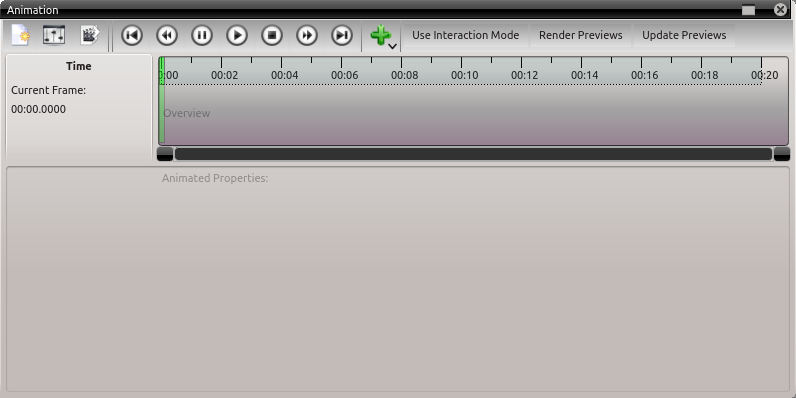
\includegraphics[scale=0.5,keepaspectratio=true]{./images/animation_window.png}
 % animation_window.png: 796x399 pixel, 90dpi, 22.47x11.26 cm, bb=0 0 637 319
 \caption{The animation window with an empty animation}
 \label{fig:animation_window}
\end{figure}

The animation editor consists of three basic parts. The first part is the animation tool bar, which is located at the top of the editor. Below the tool bar is the 
animation timeline, which provides an overview of the animation. The bottom part displays information and settings, depending on the current state of the animation
editor. 

\subsection*{Creating a Basic Animation}
To animate a property, click on the `+'-button in the middle of the animation tool bar. It will open a menu where you can select one of the groups 
which are present in the property list window. Within the group, you can select one of the properties of that group. Clicking on the property will add 
it to the list of animated properties. If no animated property has been present in the animation before, the editor will also add a \emph{keyframe} to the
timeline. \textbf{Please note that only properties which have been added to the application mode configuration (see \url{http://www.uni-muenster.de/Voreen/documentation/user_interface.html}) of the current workspace can be added to the animation.}

Basically every property which is present in the application mode configuration can be added to the animation and be animated by setting a state for the property
in each of the animation keyframes. When playing back the animation, the current value for each frame is generated by interpolating between adjacent keyframes and 
setting it to the actual properties of the workspace, so that the result can directly be seen in the quad view rendering.

After adding the first property to the animation, the animation window should look similar to the one depicted in figure \ref{fig:animation_keyframe}.

\begin{figure}[!htb]
 \centering
 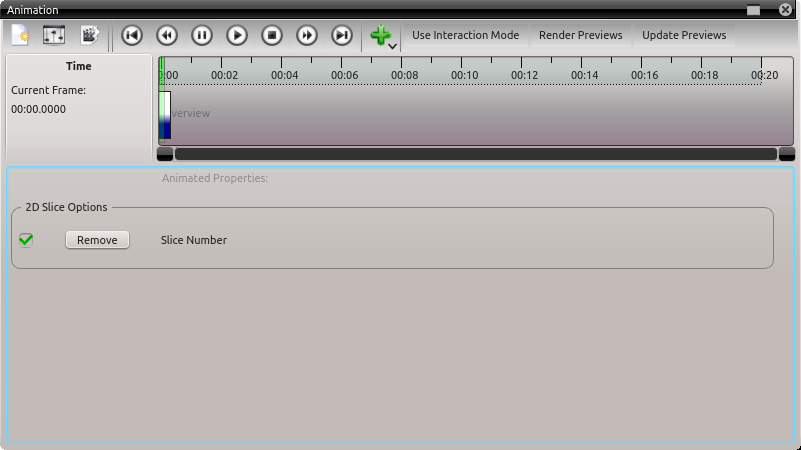
\includegraphics[scale=0.5,keepaspectratio=true]{./images/animation_keyframe.png}
 % animation_keyframe.png: 801x450 pixel, 90dpi, 22.61x12.70 cm, bb=0 0 641 360
 \caption{The animation window after a property has been added}
 \label{fig:animation_keyframe}
\end{figure}

The area at the bottom of the animation window now displays a list of all of the animated properties for each group. The property can be removed from the animation by using the 
`\verb|Remove|'-button. However, this will erase all of its animation state from the animation. By clicking the checkbox to the left of the button, animating the property
can be deactivated while still keeping the values set to the animation keyframes. Clicking on the checkbox of a deactivated property will activate its animation again.

By clicking on the keyframe in the timeline, it can be selected. This will change the layout of the bottom section of the animation window so that the value of each  
animated property can be edited for this keyframe. An example of this with two animated properties is depicted in figure \ref{fig:animation_keyframe_editing}.

\begin{figure}[htb]
 \centering
 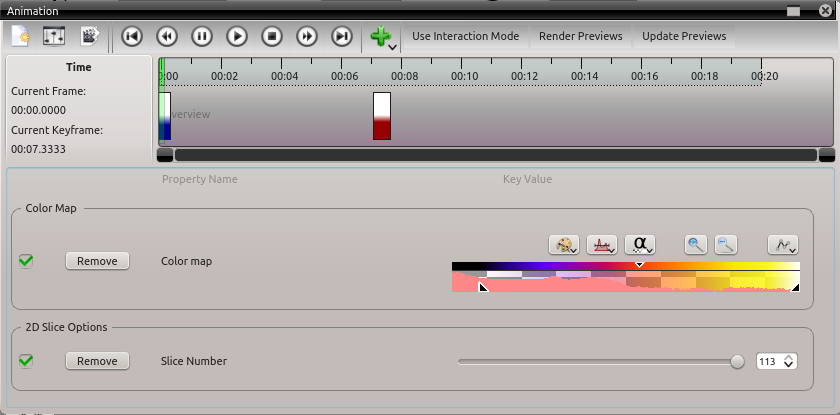
\includegraphics[scale=0.5,keepaspectratio=true]{./images/animation_keyframe_editing.png}
 % animation_keyframe_editing.png: 840x415 pixel, 90dpi, 23.71x11.71 cm, bb=0 0 672 332
 \caption{Editing the property values of a keyframe}
 \label{fig:animation_keyframe_editing}
\end{figure}

To add another keyframe to the animation, right-click on the lower part of the animation timeline (i.e. the part where the keyframes are located) and select either
`\verb|Add Keyframe|' or `\verb|Take Snapshot|'. The first option will create a keyframe, where the values for all of its animated properties are computed by interpolating 
between the keyframes already present (or using the value of the first or last keyframe, if the new keyframe is inserted as the first or last in the timeline). The 
second option will use the values currently set in the \Voreen application and record those to a keyframe. This is especially useful for three-dimensional camera settings,
as you can position the camera and then record the state to the animation.

By clicking on a keyframe and holding the left mouse button, the keyframe can be moved in the timeline. Right-clicking on a keyframe opens a menu where the keyframe 
can be removed from the animation or a snapshot of the current application settings can be recorded to the existing keyframe, overwriting its former values.

Clicking with the left mouse button in the space between two keyframes in the timeline allows to select the interval between those keyframes. 
An example of this is depicted in figure \ref{fig:animation_interval}.
\begin{figure}[!htb]
 \centering
 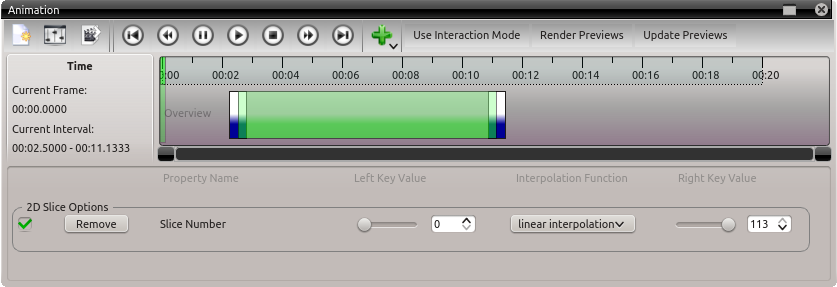
\includegraphics[scale=0.5,keepaspectratio=true]{./images/animation_interval.png}
 % animation_interval.png: 837x287 pixel, 90dpi, 23.62x8.10 cm, bb=0 0 670 230
 \caption{Selecting an interval between two keyframes of the animation}
 \label{fig:animation_interval}
\end{figure}
Selecting an interval, similar to selecting a single keyframe, allows to change the value of each of the animated properties for both the left and right keyframe.
Additionally, you can change the interpolation function that is used to interpolate between the keyframes within the interval. In most cases, the default linear 
interpolation will be sufficient. For camera animations, however, a \emph{spherical linear interpolation} should be selected.\footnote{The same
usually goes for the orientation of a clipping plane.} For a simple rotation of the camera around one axis, two keyframes with identical position and orientation (e.g., created by recording the same state twice using the `\verb|Take Snapshot|'-function) can be used with a `\verb|Rotation|'-interpolation.

The top part of the animation timeline allows to set the \emph{frame marker} to a specific time by clicking on it with the left mouse button. This will also set
the state of the animation at this time to the application, so that it allows to inspect the state of the animated properties at a specific time of the animation
directly using the quad view. Holding the left mouse button while moving in the top part of the animation timeline allows to scan through the animation, while
the state of the animated properties is directly set to the application properties. Figure \ref{fig:animation_marker} shows an example of this.

\begin{figure}[htb]
 \centering
 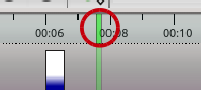
\includegraphics[scale=0.8,keepaspectratio=true]{./images/animation_marker1.png}
 % animation_marker1.png: 201x90 pixel, 96dpi, 5.32x2.38 cm, bb=0 0 151 67
 \caption{Clicking in the top part of the timeline (marked by the red circle) will set the current frame.}
 \label{fig:animation_marker}
\end{figure}

\subsection*{The Animation Tool Bar}

The leftmost icon of the animation tool bar will create a new, empty animation. However, this will erase all of the animation settings currently 
present. Animations are part of the workspace setting. It is therefore necessary to save the workspace if you want to save the animation. Animations
cannot be saved independently, as they operate on the workspace-specific properties and settings.

\begin{figure}[!htb]
 \centering
 
\includegraphics[scale=0.7,keepaspectratio=true]{./images/animation_toolbar.png}
 % animation_toolbar.png: 735x32 pixel, 90dpi, 20.75x0.90 cm, bb=0 0 588 26
 \caption{The animation tool bar}
 \label{fig:animation_toolbar}
\end{figure}

The second tool bar icon opens an animation settings dialog, which is depicted in figure \ref{fig:animation_settings}. In this dialog, you can set the duration
of the animation, i.e. the length of the animation timeline where keyframes can be placed. By selecting the `\verb|Apply Time Stretch|'-checkbox, the current
animation is scaled to fit the new duration. This can be useful to speed up or slow down an already existing animation.

\begin{figure}[htb]
 \centering
 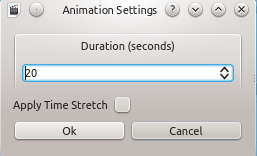
\includegraphics[scale=0.7,keepaspectratio=true]{./images/animation_settings.png}
 % animation_settings.png: 257x156 pixel, 90dpi, 7.25x4.40 cm, bb=0 0 206 125
 \caption{The animation settings dialog window}
 \label{fig:animation_settings}
\end{figure}

Next to the animation settings icon is the export icon, which opens the export dialog window depicted in figure \ref{fig:animation_export}. 
It allows to export the animation as a frame sequence, i.e. a sequence of `\verb|*.png|'-image files, or as a video file\footnote{The video export function is only present if the \texttt{ffmpeg}-module has been included in the \Voreen-build.}, and offers several configuration
options for the export format, quality and compression.

\begin{figure}[!htb]
 \centering
 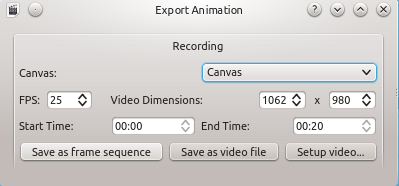
\includegraphics[scale=0.7,keepaspectratio=true]{./images/animation_export.png}
 % animation_export.png: 399x186 pixel, 90dpi, 11.26x5.25 cm, bb=0 0 319 149
 \caption{The animation export window}
 \label{fig:animation_export}
\end{figure}

Next to the export icon on the animation tool bar are the animation playback control icons, which offer the functionality to play, pause, and stop the animation playback, etc.

Activating the `\verb|Use Interaction Mode|'-button will use an interaction mode with reduced rendering quality during playback to improve the rendering speed 
of the animation. The `\verb|Use Interaction Mode|'-button activates the display of a series of small images on the timeline which visualize the animation state.
The preview images are not updated automatically if the animation changes after the previews have been created. 
The user therefore has to click on the `\verb|Update Previews|'-button to update
the preview images according to the current animation state.


